
\section{Rectangular}

\begin{figure}[h]
\centering
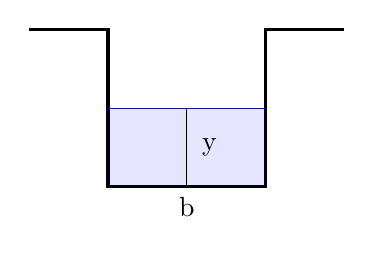
\begin{tikzpicture}
\draw[very thick] (0,0) -- (1,0) -- (1,-2)--node[below]{b}(3, -2) -- (3,0) -- (4,0);
\draw[blue] (1,-1) -- (3,-1);
\filldraw[fill=blue, opacity=0.1](1, -1) --(3, -1) -- (3, -2) -- (1,-2);
\draw (2,-2)--node[right=2]{y} (2,-1);
\end{tikzpicture}
\caption{Rectangular Section}
\end{figure}

\begin{equation}
A = by
\end{equation}

\begin{equation}
P = b + 2y
\end{equation}

\begin{equation}
R = \frac{by}{b+2y}
\end{equation}

\begin{equation}
\frac{\partial A}{\partial y} = b
\end{equation}

\begin{equation}  
f_c(y)= gb^3y^3 -Q^2b= 0
\end{equation}

\begin{equation}  
y_c^3 = \frac{Q^2}{gb^2}
\end{equation}
